% TikZ redraw for exercise 2-51
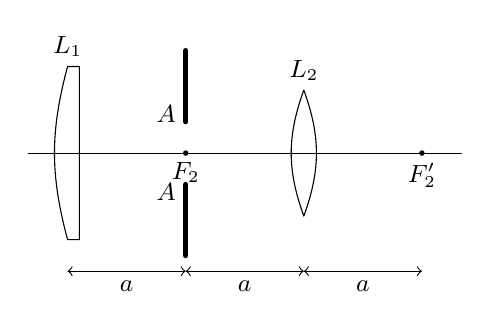
\begin{tikzpicture}[font=\small,line cap=round,line join=round]
\draw(-.5,0)--(5,0);\draw(0,-1.1)to[bend left=15](0,1.1)--(.15,1.1)--(.15,-1.1)--cycle;\draw(3,-.8)to[bend left=20](3,.8)to[bend left=20]cycle;\node[above]at(0,1.1){$L_1$};\node[above]at(3,.8){$L_2$};\draw[line width=2pt](1.5,.4)--(1.5,1.3) (1.5,-.4)--(1.5,-1.3);\node[left]at(1.5,.5){$A$};\node[left]at(1.5,-.5){$A$};\fill(1.5,0)circle(1pt)node[below]{$F_2$};\fill(4.5,0)circle(1pt)node[below]{$F'_2$};\foreach\a/\b in {0/1.5,1.5/3,3/4.5}\draw[<->](\a,-1.5)--node[below]{$a$}(\b,-1.5);
\end{tikzpicture}
